\documentclass{sig-alternate}
\usepackage{graphicx}
\usepackage{eepic}

\begin{document}

\conferenceinfo{DEBS}{2009 Nashville, Tennessee USA}

\title{Passing Actor Continuations}
\subtitle{Efficient and Extensible Request Routing for Event-Driven Architectures}

\numberofauthors{1} 

\author{
\alignauthor
Stefan Plantikow\\
       \affaddr{Zuse Institute Berlin (ZIB)}\\
       \affaddr{Takustrasse 7}\\
       \affaddr{14195 Berlin, Germany}\\
       %\email{plantikow@zib.de}
}

\date{1 March 2009}


\maketitle

\begin{abstract}

The request routing logic between the different stages in event-driven architectures is often
distributed over different portions of the source code. This can make it hard to change and
understand the flow of events in the system.

The article presents an approach that allows writing request routing logic as a set of routing
scripts. Requests are executed step-wise according to their script by sending continuations that
encapsulate their request's current execution state to stages for local processing and optional
forwarding of follow-up continuations. The implementation of a domain specific language for routing
scripts for the scala actor library is described and evaluated. The results indicate that request
routing with actor continuations performs about equally or better to using separate stages for
request routing logic for scripts of at least 3 sequential steps.

\end{abstract}

\category{H.2.4}{Information Systems}{Systems}[Concurrency]         
\category{D.1.3}{Software}{Programming Techniques}[Concurrent Programming]         
\category{D.3.3}{Programming Languages}{Language Constructs and Features}[Concurrency]
%\category{D.2.11}{Software Engineering}{Distribution, Maintenance, and Enhancement}[Extensibility]

\keywords{Request Routing, Event-Driven Architecture, Partial Continuation, Actor Model, Scala}


\section{Introduction}             

Using a staged, event-driven architecture is an approach to the design of server software that can 
provide high degrees of concurrency and throughput.  This is achieved by structuring the software as
a set of stages that communicate exclusively via event queues and by optionally performing admission 
control on each queue.  

% // TODO Examples of staged architectures are ...
% // TODO XtreemFS example

Depite their benefits, event-driven architectures can lead to a distribution of application logic
over different stages. The implementation of each stage usually resides in a different portions of
the source code and therefore the dynamic routing of requests through different stages is not
described by a single source location.

This reduces the understandability of the system and in turn makes it harder to modify the request
routing logic. Additionally, it makes it difficult to add new request types without changing the
source code of existing stages and redeploying the system.

- Problem deScription\\

- Article overview\\
                                
                         
\section{Preliminaries}

-Actor Model \\

Scala is a multiparadigm programming language for the Java virtual machine that fuses objectoriented
and functional techniques. Since Scala is statically typed, its compiler produces considerably fast
code. At the same time, the languages includes features that are often only found in dynamically
typed languages for the JVM. Sofleuse uses some of those, like CPS-transform in
generator-expressions, anonymous functions, multiple inheritance, singleton objects and self-types.

Additionally, the Scala standard library includes a rich set of concurrency primitives that
implement different process calculi, like the join-calculus, the pi-calculus, and the actor model.
Actors are available in two flavours: \textbf{react}-actors who get scheduled by the actor library
piece-wise to different threads, and \textbf{receive}-actors that live in their own thread. Since
stage-based architecture associates one thread with each stage, for the purposes of this article, 
only \textbf{receive}-based actors are considered.



\section{Request Routing}

The application logic of event-driven architectures can be devided into two categories. The first
category, processing logic, is the part of application logic that necessarily must be executed at a
specific stage in order to access resources or state that are only available locally. The second
category, the request routing logic, describes how a given incoming request is handled by executing
interdependent processing logic at many stages.

Often, routing logic is contained implicitly in the event handling of single stages and the
follow-up events created by them. This implicit containment leads to difficulties in understanding
and modifying those systems.

Additionally, request routing logic may be stateful, i.e. the result of executing processing logic
at some stage may determine how and at which stages request handling needs to be continued. This
places further burdens on the implementation of single stages, as incoming- and outgoing events have
to be amended with request state, although it might be completely independent from the intended
purpose of the stage.

To give an example, imagine a simple system for launching satellites into space. Incoming
reqeuests are amended with authentication information in the first stage. In the second stage, this
information is then used to authorize the request and eventually launch the rocket. Only after the
satellite has begun to operate, some third stage (i.e. the press office) is informed.  Now, imagine
that the initial request needs to be amended with extra information (name and owner of satellite)
for the press office.  Passing this information down requires modifying the events to and from
the rocket launching stage with fields for the additional payload, although this extra information
is of no importance to launching the rocket.

This intertwining of processing and request routing logic is a case of insufficient separation of
concerns, calling for a different way to describe both types of application logic.  Next, two 
different approaches that address this issue are described.


\subsection{Ping-Pong Approach}

A straightforward way to deal with this problem is to transfer the execution of the request routing
logic to a separate stage. Requests enter the system as separate events at such a routing stage.
This stage then continously forwards events to some stage, waits for a reply, and upon receipt,
decides how to continue based on this and previous reply-events for the request. In the following,
this will be called the ping-pong-approach.

While this approach allows to write the event flow portion of the application logic in a single
stage, it has two disadvantages: First, it requires the creation of additional stages and the
associated computational overhead. Second, and more importantly, it results in extra messages
between request routing and regular processing stages.

The \emph{ping-pong (PPNG)} approach centralizes routing logic in a single place by introducing an
additional stage. This can be understood as the consolidation of a control flow that otherwise would
be scattered throughout the source code. Additionally, for each request, the routing stage stores
intermediate results and associated state for reuse by later events, as well as provides the ability
to pause a request's control flow while waiting for the execution of processing logic by some other
stage.



\subsection{Passing Actor Continuations}

Extracting routing logic requires a mechanism for pausable, stateful control-flow. Introducing an
extra stage is just one way to achieve this. Other possible techniques are the use of coroutines or
continuations the latter on which this article concentrates.

The \emph{continuation} of a computation describes the part of a computation that yet needs to be
computed. Some programming languages, especially the scheme-dialect of lisp, provide means for
explicitly capturing the continuation at runtime and by this allow it to be executed arbitrary
times. This can be used to implement new control structures inside the programming language.

// Parameterization\\

This ability may be used to create pausable, stateful control-flow: Each stage only processes
messages that actually are anonymous functions that represent the current continuation of some
request. Such incoming continuations are executed by calling them with the executing stage as their
sole argument. Through this means, request continuations gain access to the functionality of local
stages.

When the execution of a request continuation at a stage is about to finish, the follow-up 
continuation may be captured in a last step.  This follow-up continuation is then simply sent
to the next stage where request handling continues.  

This \emph{actor continuation passing (ACP)} approach does not require any intermediate stages for
the execution of the request logic and through this avoids the additional messages of the ping-pong
approach. It is also stateful, since continuations contain all of their stack frame at
capture time. On the downside, it requires some overhead for continuation capturing. The impact of
these different properties will be shown in the evaluation section.

                         



\section{Sofleuse: A Request Routing DSL}

Now a framework based on actor continuation passing, Sofleuse, is presented. Sofleuse has been
implemented in the Scala programming language using the scala actor's library. Sofleuse provides a
\emph{domain specific language (DSL)} for writing routing scripts that execute over a set of locally
running actors.

Routing scripts are implemented by subclassing the class Play and overriding the apply method. Play
instances are provided with a set of DSL-commands for writing scripts. Commands provide the ability
to structure scripts as a sequence of blocks that are each executed at different stages. To capture
continuations, commands are chained by using scala's CPS-transforming \textbf{for}-generator-expressions
(explained below). The following command set is provided:


\begin{itemize}                                   
	\item \textbf{\emph{v} <- remember(\emph{value})} Bind \emph{value} to \emph{v} for reuse by
	later routing decisions of the script
	\item \textbf{\emph{v} <- compute(\emph{thunk})} Compute \emph{thunk} at the current local stage.  
	The return value is bound to \emph{v} and may be reused in later routing decisions of the script
	%\item \textbf{\emph{v} <- computeWith(\emph{o})(\emph{thunk})} Like \textbf{compute(\emph{thunk})} 
	%but \emph{thunk} takes \emph{o} as its first argument
	\item \textbf{\emph{s} <- goto(\emph{stage})} Continue execution at stage \emph{stage} and 
	return a reference \emph{s} for gainining access to the local processing logic of \emph{stage} 
	(usually \emph{stage} itself)
	\item \textbf{\emph{s} <- jump(\emph{thunk})} Execute thunk at the current (active) stage in 
	order to determine the next stage for script execution.	Return a suitable reference \emph{s} to 
	gain access to the local processing logic of that stage
	%\item \textbf{\emph{t} <- cast[\emph{T}](\emph{stage})} Like \textbf{goto(\emph{stage})} but 
	%cast the result of \textbf{goto(\emph{stage})} to type \emph{T}   
	\item \textbf{yield(result)} The yield statement of the \textbf{for}-expression may optionally be used to 
	return a result to the initial caller of the script                           	
	%\item \textbf{endOfPlay} Syntactically denote the end of a routing script that does not return
	% a value to its caller.
\end{itemize}


The class Play places an upper bound on the type of actor-stages over which the routing script
commands operate. Routing scripts can also be written directly as \textbf{for}-expressions without
using class Play. This may lead to more typecasts through the use of the untyped DSL-commands
provided as additional utility functions by Sofleuse. Routing scripts based on
\textbf{for}-expressions using two additional commands of the DSL:

\begin{itemize}
    \item \textbf{run(\emph{forExpr})} Run \emph{forExpr} and wait until its execution yields a result (blocks current actor)
	\item \textbf{asyncRun(\emph{forExpr})} Runs \emph{forExpr} without waiting for a result (non-blocking)
\end{itemize}	

As an example, consider the execution of a single remote procedure call~(Fig.~\ref{fig:rpc}). The
call is wrapped as a function that initially creates a new script based on a simple
\textbf{for}-expression. The script itself first transfers the execution to the \emph{targetStage}
for the RPC using \textbf{goto}. Then, the actual RPC is executed at that stage using
\textbf{compute}, and finally a return value is yielded. To actually execute this routing script, it
is started with \textbf{run}.

\begin{figure}
\centering    
{\footnotesize\begin{tabular}{l}           
$\textbf{def}\ $rpc$(\emph{targetStage}, \emph{args})\ =\ \{$\\	
\hspace{2ex} $\textbf{val}\ \emph{request}\ =\ \textbf{for} ($\\
\hspace{6ex} $\emph{stageRep}\ \leftarrow\ $goto$(\emph{targetStage})$\\
\hspace{6ex} $\emph{procResult}\ \leftarrow\ $compute$\ \{\ stageRep.$proc$(\emph{args})\ \}$\\
\hspace{2ex} $)\ \textbf{yield}\ procResult$\\
\hspace{2ex} $\textbf{return}\ $run$(\emph{request})$\\   
$\}$\\
\end{tabular}}
\caption{Simple RPC in Sofleuse\label{fig:rpc}}
\end{figure}

\begin{figure*}[t]
\begin{center}
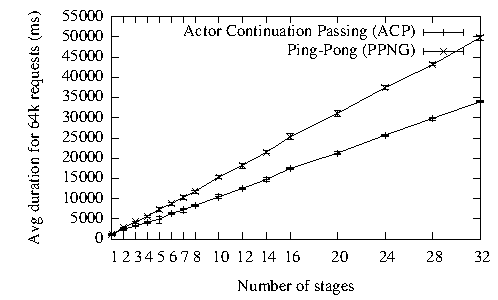
\includegraphics[width=.33\hsize]{plots/BENCHMARK-8CORE-2009-03-01-23:59-LIN.pdf}%
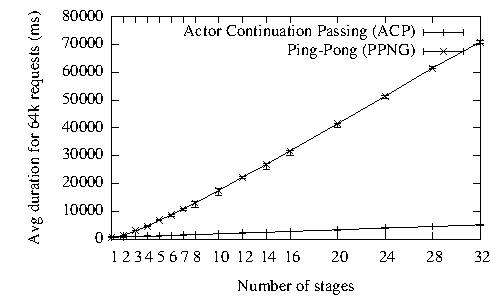
\includegraphics[width=.33\hsize]{plots/BENCHMARK-8CORE-2009-03-01-23:59-BLK.pdf}%
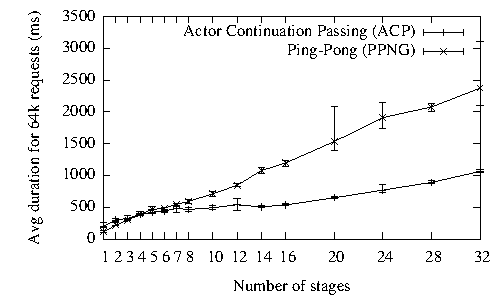
\includegraphics[width=.33\hsize]{plots/BENCHMARK-8CORE-2009-03-01-23:59-ALL.pdf}
\end{center}
\end{figure*}
	

\section{Implementing ACP}

In the following, the actor continuation passing approach to the extraction of request routing logic
into request routing scripts is described.
                             

\subsection{Actors that execute arbitrary code} 

First, it is necessary that actors may be instructed externally to execute thunks of arbitrary
control flow. For this, Sofleuse provides the trait StageActor whose main loop listens for messages
consisting of one-argument anonymous lambda-functions. When such a function is received, it is
executed by passing a reference to the StageActor itself as its first argument to grant access to 
the local processing logic.

Additionally, for advanced uses, Sofleuse supports another type of actor, whose processing logic
representation (called Prop) can be replaced at runtime by routing scripts.


\subsection{Passing Actor Continuations}

Using StageActor itself already is sufficient to implement request routing based on partial
continuations. To do so, anonymous lambda functions that reify the current continuation need to be
explicitly written out in the source code and sent to the StageActor via normal message passing.
However, this leads to a nesting level of anonymous lambda functions that is as large as the number
of sequentially passed stages, and fixes the message sending mechanism that is used in request
routing scripts.

\emph{Continuation Passing Style (CPS)} is a control flow graph transformation from the field of
compiler construction that eliminates function return values by replacing them with an additional
continuation parameter. The continuation parameter is invoked inside the function with a
concrete return value as its argument.

Request routing with actor continuation passing can be implemented through CPS-transform and
message sending at stage boundaries.  A routing script is written as a sequence of code blocks.
Each code block runs at the local stage and computes the follow-up stage for the next block.
This follow-up stage may be bound to a variable such that its processing logic may be accessed
by its successor.

All blocks are CPS-transformed such that each block is provided with a continuation that is
parameterized with the follow-up stage. If this continuation is called, the remaining blocks are
executed. Usually, this will be the last step of a block. However, instead of directly executing the
continuation inside the normal control flow (and therefore the current stage's thread), the 
continuation is sent as a message to the follow-up stage for deferred execution.


\subsection{CPS-Transform in Scala}     

Sofleuse exploits Scala's \textbf{for}-generator-expressions to implement CPS-transform. Routing
scripts are written as expressions of the form:

   
\medskip
{\footnotesize\begin{tabular}{l} $\mathbf{for}\ (\mathit{v_1} \leftarrow \mathit{e_1}, \mathit{v_2} \leftarrow
\mathit{e_2}, \ldots, \mathit{v_n} \leftarrow \mathit{e_n})\ \mathbf{yield}\ \mathit{r}$
\end{tabular}}
\medskip


This iterates sequentially from outmost to innermost over the generators $e_i$. Each $v_i$ is
consecutively bound to the values produced by its generator $e_i$. Results are created by evaluating
$r$ in each iteration until $e_1$ is exhausted.

Scala abstracts from how \textbf{for} interprets different types of generators by CPS-transforming
the expression and calling abstract methods on the generators. For example, above expression is
transformed by the Scala compiler into:


\medskip
{\footnotesize\begin{tabular}{l}
$\mathit{e_1}.$flatMap$\ \{\ \mathbf{case}\ \mathit{v_1}\ \Rightarrow$\\
$\hspace{2ex}\mathit{e_2}.$flatMap$\ \{\ \mathbf{case}\ \mathit{v_2}\ \Rightarrow\ \ldots\ \mathit{e_n}.$map$\ \{\ \mathit{r}\ \}\ \ldots\ \}\ \}$
\end{tabular}}
\medskip


Every $\{\ \mathbf{case}\ \mathit{v_i}\ \Rightarrow\ \ldots\ \}$ is an anonymous lambda function
that reifies the continuation for the remaining \textbf{for}-generator-expression.\footnote{Scala
supports complex pattern matching, therefore the lambda is written here with a pattern-matching
\textbf{case}-statement, although this feature is not used in above example} To make this implicit
CPS-transformation usable, the scala standard library contains the abstract class Responder which
provides implementations of flatMap and map in terms of a function respond. Respond takes the
continuation for the remaining generator-expression as its only argument, generates values, and
iterates by calling the continuation with them.

To implement actor continuation passing, Sofleuse associates each StageActor with a Responder whose
respond method simply forwards passed continuations to the StageActor via message passing:
                                                                                            
\medskip
{\footnotesize\begin{tabular}{l}                                
$\mathbf{object}\ $responder$\ \mathbf{extends}\ $Responder[this.type]$\ \{$\\
\hspace{2ex}$\mathbf{def}\ $respond$(\mathit{k}:\ $Actor.this.type$\ \Rightarrow\ $Unit$):\ $Unit$\ =\ $self.send$(\mathit{k})$\\
$\}$\\
\\
$\mathbf{def}\ $asResponder$:\ $Responder[Actor.this.type]$\ =\ $responder\\
\end{tabular}}
\medskip

This mechanism is sufficient to implement the Sofleuse DSL. \textbf{goto} returns a responder for
its argument as described above. \textbf{remember} simply creates a constant responder for a single
value. \textbf{run} uses the actor library to create a dedicated channel for return values. All
other commands are implementable on top of goto and remember.

                                                       
\subsection{Limitations}

To avoid stack overflow, CPS-transform is often used in conjunction with tail call optimization
(TCO). Since message passing switches between stacks of different threads and Sofleuse is targeted
for writing routing scripts that are bounded in the number of stages by a small constant, Sofleuse
currently does not perform TCO.
    
Sofleuse currently does not yet support exception handling across stage boundaries.

The strictly linear nature of generator expressions makes writing routing scripts with
non-linear control-flow more difficult and may require the execution of routing sub-scripts.  
However, even in such a scenario all request routing logic is written in a single routing
script.



\subsection{Continuation Access}

Sofleuse includes an extended version of StageActor that allows routing scripts to 
access the currently running continuation.  This may be used to forward continuations
to other stages (load balancing) or execute the same continuation repeatedly over multiple
actors (replication).                               

% Additionally, scripts may register a hook that will be executed with the next continuation as its
% argument as soon as it arrives. This is useful for implementing functions like
% shutdownAfterNextScene that can be called during \textbf{compute} to trigger a stage shutdown after
% the following \textbf{goto} (batches of consecutive commands to the same stage from one script 
% are always executed together without interleaving commands from other scripts). 

\section{Evaluation}
               
Both approaches have been evaluated in the following setting. Incoming requests have to be

// Describe settting

// Present results

// Discuss in detail esp w regard to actor library


\section{Related Work}

// Let's see...

\section{Summary}
                  
// Fazit

// Interesting applications

\section{Acknowledgments}

\bibliographystyle{abbrv}
%\bibliography{sigproc}  

\end{document}
